\section{Resultados e discussão}

Para encontrar todos os resultados necessários para comprovar a teoria, a prática foi dividida em algumas etapas, sendo elas:


\begin{itemize}

    \item Com apoio do aporte teórico realizado durante a prática, foi montado o circuito da figura \ref{ckt:1}, e medidos os parâmetros de cada onda nos pontos $V_{o1}$ e $V_{o2}$;
    
    \item Após isso foi substituído a resistência $R_3$ de $8.2 \times10^3$ \ohm, por um resistor de $4.7 \times10^3$ $\ohm$ em série com um potenciômetro de $50 \times10^3 $ \ohm, verificando e discutindo os resultados encontrados.
    
    \item Por fim, foi devolvido o valor padrão de $8.2 \times10^3$ $\ohm$ a $R_3$ e agora foi colocado o potenciômetro em série com $R_2$, anotando e discutindo os resultados observados.  
\end{itemize}

Antes dos circuitos serem montados, os diodos zeners foram testados separadamente para garantir que não estejam funcionando na região de ruptura. Só assim foi montado o circuito da figura \ref{ckt:1}.

Não foi possível a utilização do potenciômetro de $10 \times10^3 $ $\ohm$, pois o mesmo não havia em laboratório no momento da realização da prática, foi substituído por um potenciômetro por um de $50 \times10^3 $ $\ohm$.   

Com a utilização do osciloscópio foram verificadas as formas de onda de $V_{o1}$ e $V_{o2}$, espera-se que em $V_{o1}$ seja uma onda quadrada, e que sua amplitude fique em torno de $\pm 3.4V$. Já espera-se que em $V_{o2}$ seja uma onda triangular já que vamos integrar a saída quadrada de circuito comparador com histerese, e sua amplitude seja em torno de $\pm 2.32V$. A sua frequência gira em torno de $2.02$ kHz

\begin{figure}[H] 
\centering
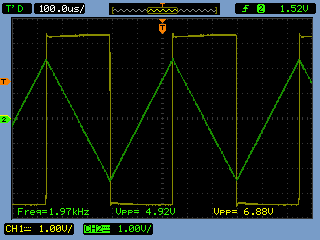
\includegraphics[width=8cm]{images/vo12.png}
\caption{Formas de onda de $V_{o1}$ (CH1) e $V_{o2}$ (CH2) do gerador de onda triangular.}
\label{fig1} 
\end{figure}

Podemos notar que pelos resultados encontrados acima, e considerando os erros associados a parte prática. Condizem bastante com o descrito na parte teórica.

Substituindo a resistência fixa de $8.2 \times10^3$ \ohm, por uma resistência de $4.7 \times10^3 $ $\ohm$ em série com um potenciômetro de $50 \times10^3 $ \ohm, obtemos uma comparação máxima e mínima, de acordo com os valores máximo e mínimos do potenciômetro. O que é observado nas figuras abaixo.

\begin{figure}[H] 
\centering
\subfigure[ref1][Valor Mínimo.]{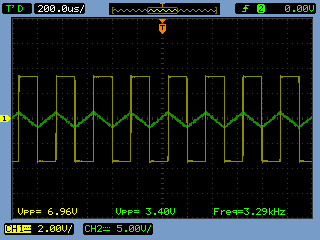
\includegraphics[width=7.6cm]{images/pmin.png}}
\subfigure[ref2][Valor Máximo.]{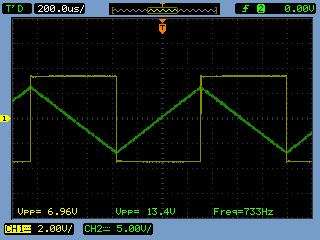
\includegraphics[width=7.6cm]{images/pmax.png}}
\caption{Formas de ondas para $V_{o1}$ e $V_{o2}$ variando-se o novo $R_3$.}
\label{cut}
\end{figure}

Podemos perceber que ao variar o potenciômetro, muda-se a frequência e amplitude da onda de forma proporcional de modo que a inclinação da onda triangular é sempre a mesma de forma que em todos os casos observados é possível observar esse efeito. Isso só é possível devido se mudarmos o valor da resistência $R_3$ iremos modificar o valor da amplitude da tensão $V_{o2}$, consequentemente, o valor da frequência de oscilação do sinal.

Já na configuração em que colocamos um potenciômetro de $50 \times10^3 $ $\ohm$ em série com $R_2$, mantendo $R_3 = 8.2 \times10^3$ \ohm, de modo a obter uma comparação máxima e mínima, de acordo com os valores máximo e mínimos do potenciômetro. Podemos observar essas mudação nas figuras a seguir.

\begin{figure}[H] 
\centering
\subfigure[ref1][Valor Mínimo.]{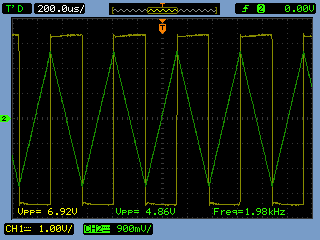
\includegraphics[width=7.6cm]{images/r2_min.png}}
\subfigure[ref2][Valor Máximo.]{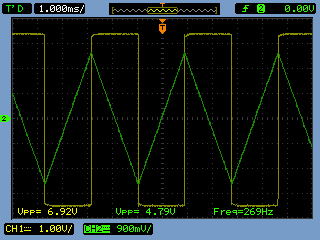
\includegraphics[width=7.6cm]{images/r2_max.png}}
\caption{Formas de ondas para $V_{o1}$ e $V_{o2}$ variando-se o novo $R_2$.}
\label{cut}
\end{figure}

Nota-se que ao variar o valor da resistência $R_2$ com o potenciômetro, vamos modificar o valor da inclinação da onda triangular $V_{o2}$, somente o valor
da frequência de oscilação do sinal mudará, ou seja, o período da onda quadrada mudará, mas amplitude, tanto da onda quadrada quanto da triangular, não mudarão, como esperado na analise teórica.

%\newpage